\documentclass[tikz,border=6pt]{standalone}

\usepackage{tikz}
\usepackage{xcolor}
\usetikzlibrary{arrows.meta, positioning, fit, backgrounds, calc}

% ── Palette (Tol bright, matches every other figure in the paper) ────────────
\definecolor{colBlue}{HTML}{0077BB}
\definecolor{colTeal}{HTML}{009988}
\definecolor{colOrange}{HTML}{EE7733}
\definecolor{colRed}{HTML}{CC3311}
\definecolor{colGray}{HTML}{444444}

\tikzset{
  % Pipeline step boxes (top row)
  pbox/.style={
    draw, very thick, rounded corners=5pt,
    align=center, inner sep=9pt,
    minimum width=3.0cm, minimum height=1.5cm,
    font=\small,
  },
  pA/.style={pbox, draw=colBlue!80!black,   fill=colBlue!10},
  pB/.style={pbox, draw=colTeal!80!black,   fill=colTeal!10},
  pC/.style={pbox, draw=colOrange!80!black, fill=colOrange!12},
  pD/.style={pbox, draw=colOrange!80!black, fill=colOrange!12},
  % Artifact nodes (rounded rectangles, smaller)
  art/.style={
    draw, thick, rounded corners=10pt,
    align=center, inner sep=7pt,
    minimum width=2.4cm, minimum height=0.9cm,
    font=\small,
  },
  artBase/.style={art, draw=colRed!70!black,   fill=colRed!8},
  artLora/.style={art, draw=colBlue!70!black,  fill=colBlue!8},
  % Evaluation condition boxes
  ebox/.style={
    draw, very thick, rounded corners=4pt,
    align=center, inner sep=7pt,
    minimum width=2.8cm, minimum height=1.1cm,
    font=\small,
  },
  eBase/.style={ebox, draw=colRed!80!black,   fill=colRed!8},
  eLora/.style={ebox, draw=colBlue!80!black,  fill=colBlue!8},
  % Holdout node
  holdout/.style={
    draw, very thick, rounded corners=4pt,
    align=center, inner sep=8pt,
    minimum width=5.5cm, minimum height=1.2cm,
    font=\small,
    draw=colRed!70!black, fill=colRed!7,
  },
  % Arrows
  arr/.style={-{Latex[length=2.8mm,width=2mm]}, very thick, colGray},
  arrthin/.style={-{Latex[length=2.2mm,width=1.6mm]}, thick},
  % Region brackets
  region/.style={draw, dashed, thick, rounded corners=7pt, inner sep=10pt},
}

\begin{document}
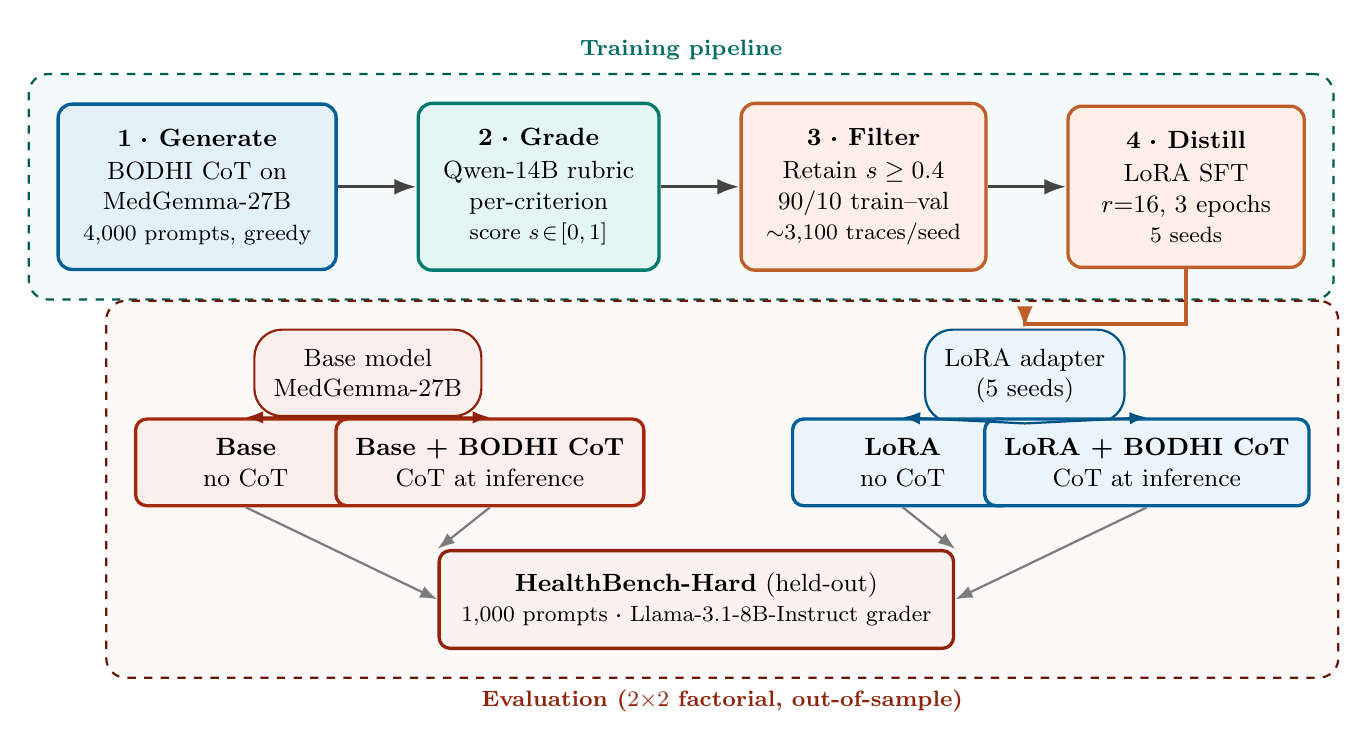
\begin{tikzpicture}

%% ═══════════════════════════════════════════════════════════════════════════
%% TOP ROW – Training pipeline
%% ═══════════════════════════════════════════════════════════════════════════

\node[pA] (s1) at (0,0) {
  \textbf{1 · Generate}\\[1pt]
  BODHI CoT on\\
  MedGemma-27B\\
  {\footnotesize 4,000 prompts, greedy}
};

\node[pB, right=10mm of s1] (s2) {
  \textbf{2 · Grade}\\[1pt]
  Qwen-14B rubric\\
  per-criterion\\
  {\footnotesize score $s\!\in\![0,1]$}
};

\node[pC, right=10mm of s2] (s3) {
  \textbf{3 · Filter}\\[1pt]
  Retain $s \geq 0.4$\\
  90/10 train--val\\
  {\footnotesize $\sim$3,100 traces/seed}
};

\node[pD, right=10mm of s3] (s4) {
  \textbf{4 · Distill}\\[1pt]
  LoRA SFT\\
  $r{=}16$, 3 epochs\\
  {\footnotesize 5 seeds}
};

\draw[arr] (s1) -- (s2);
\draw[arr] (s2) -- (s3);
\draw[arr] (s3) -- (s4);

%% ═══════════════════════════════════════════════════════════════════════════
%% MIDDLE ROW – Base model  |  LoRA adapter
%% Both sit at the same y-level; adapter is directly below step 4
%% ═══════════════════════════════════════════════════════════════════════════

% Compute the horizontal midpoint of boxes 1+2 (for base model)
% s1 center ≈ 0, s2 center ≈ 3.0+1.0 = 4.0 → mid ≈ 2.0 cm
% We'll use a calculated x: midpoint of s1 and s2 centers
\coordinate (midS1S2) at ($(s1)!0.5!(s2)$);
\coordinate (midS3S4) at ($(s3)!0.5!(s4)$);

\node[artBase, below=18mm of midS1S2] (base) {
  Base model\\
  MedGemma-27B
};

\node[artLora, below=18mm of midS3S4] (adapter) {
  LoRA adapter\\
  (5 seeds)
};

% Arrow: step 4 → adapter
\draw[arr, colOrange!80!black] (s4.south) -- ++(0,-7mm) -| (adapter.north);

%% ═══════════════════════════════════════════════════════════════════════════
%% BOTTOM ROW – 2×2 evaluation conditions
%% Positioned symmetrically: base conditions left, LoRA conditions right
%% ═══════════════════════════════════════════════════════════════════════════

% y-level for eval boxes: below both artifact nodes
\coordinate (evalY) at ($(base.south)+(0,-17mm)$);

% Horizontal centers: left pair centered under base model, right pair under adapter
% base center ≈ midS1S2 x, adapter center ≈ midS3S4 x
\coordinate (lc) at ($(midS1S2)+(0,0)$);  % left-pair center
\coordinate (rc) at ($(midS3S4)+(0,0)$);  % right-pair center

% Half-separation between boxes within each pair
\pgfmathsetmacro{\hsep}{1.55}  % cm, half-gap between pair members

% Compute actual positions
\coordinate (eBasePos) at ($(lc)+(-\hsep cm,0)+(0,-17mm)+(0,-18mm)$);
\coordinate (eBCoTPos) at ($(lc)+(\hsep cm,0)+(0,-17mm)+(0,-18mm)$);
\coordinate (eLoraPos) at ($(rc)+(-\hsep cm,0)+(0,-17mm)+(0,-18mm)$);
\coordinate (eLCoTPos) at ($(rc)+(\hsep cm,0)+(0,-17mm)+(0,-18mm)$);

\node[eBase] (ebase)  at (eBasePos) {\textbf{Base}\\no CoT};
\node[eBase] (ebcot)  at (eBCoTPos) {\textbf{Base + BODHI CoT}\\CoT at inference};
\node[eLora] (elora)  at (eLoraPos) {\textbf{LoRA}\\no CoT};
\node[eLora] (elcot)  at (eLCoTPos) {\textbf{LoRA + BODHI CoT}\\CoT at inference};

% Arrows: base model → its two conditions
\draw[arrthin, colRed!70!black]   (base.south) -- (ebase.north);
\draw[arrthin, colRed!70!black]   (base.south) -- (ebcot.north);

% Arrows: adapter → its two conditions
\draw[arrthin, colBlue!70!black]  (adapter.south) -- (elora.north);
\draw[arrthin, colBlue!70!black]  (adapter.south) -- (elcot.north);

%% ═══════════════════════════════════════════════════════════════════════════
%% HOLDOUT – HealthBench-Hard, below all four eval boxes
%% ═══════════════════════════════════════════════════════════════════════════

% Position holdout centered between all four eval boxes
\coordinate (midAll) at ($(ebase)!0.5!(elcot)$);
\node[holdout, below=11mm of midAll] (hb) {
  \textbf{HealthBench-Hard} (held-out)\\
  {\footnotesize 1,000 prompts · Llama-3.1-8B-Instruct grader}
};

\draw[arrthin, colGray!70] (ebase.south) -- (hb.west);
\draw[arrthin, colGray!70] (ebcot.south) -- (hb.north west);
\draw[arrthin, colGray!70] (elora.south) -- (hb.north east);
\draw[arrthin, colGray!70] (elcot.south) -- (hb.east);

%% ═══════════════════════════════════════════════════════════════════════════
%% BACKGROUND REGIONS
%% ═══════════════════════════════════════════════════════════════════════════

\begin{scope}[on background layer]
  % Training pipeline region
  \node[region, draw=colTeal!60!black, fill=colTeal!4,
        fit=(s1)(s2)(s3)(s4),
        label={[font=\footnotesize\bfseries, text=colTeal!70!black]
               above:{\strut Training pipeline}}]
    (trainreg) {};

  % Evaluation region
  \node[region, draw=colRed!50!black, fill=colRed!3,
        fit=(base)(adapter)(ebase)(ebcot)(elora)(elcot)(hb),
        label={[font=\footnotesize\bfseries, text=colRed!70!black]
               below:{\strut Evaluation ($2{\times}2$ factorial, out-of-sample)}}]
    (evalreg) {};
\end{scope}

\end{tikzpicture}
\end{document}
